\documentclass{beamer}
\usepackage{manfnt}
\usepackage{txfonts}
\usepackage{hyperref}

\hypersetup{colorlinks=false,linkbordercolor=red,linkcolor=green,pdfborderstyle={/S/U/W 1}}

\addtobeamertemplate{navigation symbols}{}{ \hspace{1em}    \usebeamerfont{footline}%
    \insertframenumber / \inserttotalframenumber}

\geometry{papersize={12.8cm,12cm}}
\usepackage{lipsum}

\makeatletter
\newenvironment<>{contdproof}[1][\proofname]{%
    \par
    \def\insertproofname{#1\@addpunct{.}}%
    \usebeamertemplate{proof begin}#2}
  {\usebeamertemplate{proof end}}
\makeatother


\setbeamertemplate{theorems}[numbered]

\newtheorem*{nonumdefinition}{Definition}
\newtheorem*{nonumproblem}{Problem}
\newtheorem*{nonumremark}{Remark}
\newtheorem*{nonumexample}{Example}
\newtheorem*{nonumproposition}{Proposition}
\newtheorem{proposition}[theorem]{Proposition}


\usepackage{tikz}
\newcommand*\mycirc[1]{%
  \tikz[baseline=(C.base)]\node[draw,circle,inner sep=.7pt](C) {#1};\:
}


\newcommand\myheading[1]{%
  \par\bigskip
  {\color{blue}{\large #1}}\par\smallskip}

%\usetheme{Warsaw}
%\usetheme{Berkeley} %sample 1
\usetheme{Berlin} % sample 2
%\usetheme{AnnArbor} % sample 3

\let\otp\titlepage
\renewcommand{\titlepage}{\otp\addtocounter{framenumber}{-1}}



\title{Lecture 3}
\author{}
\date{}


\begin{document}
\begin{frame}[plain]
\titlepage
\end{frame}

\begin{frame}
\myheading{Probability Computations}

Pg. 67, \#42 is one of the hardest problems in the course. The answer is a simple fraction so here should be a simple way to do it. I don't know a simple way - I used the formula for $P(A\cup B\cup C)$, text pg. 56 or Lecture 1, pg. 30. If you find a simple way show it to me or your TA and you will get a ``gold star''. We will remember it when it comes to final grade time.
\end{frame}

\begin{frame}
The rest of this lecture will be about

\myheading{Bridge Hands and Poker Hands}

\myheading{Bridge Hands}

If you play bridge you get dealt a hand of 13 cards. 

Let $S$ be the set of all bridge hands (so our ``experiment'' is dealing 13 cards).

Since the order in which you receive the cards doesn't count (it never does in card games)
\begin{align*}
\sharp (S) &= \binom{52}{13}\\
           &= \text{the number of 13 element subsets of a 52 element set.}
\end{align*}
\end{frame}

\begin{frame}
We will now compute the probability of certain bridge hands.
\begin{enumerate}
\item Let $A$ = the hand is all hearts. What is $\sharp(A)$? We use the ``principle of restricted choice''. Our choice is restricted to the subset of hearts - we here to choose 13. There are $13$ hearts so we have $\binom{13}{13}=1$ hands.

So 
$$
P(A)=\dfrac{\sharp(A)}{\sharp(S)}=\dfrac{1}{\binom{52}{13}}
$$
($A$ is very unlikely)
\end{enumerate}
\end{frame}

\begin{frame}
\begin{enumerate}
\setcounter{enumi}{1}
\item Let $B$ = there are no hearts \dbend\ warning = dangerous, turn 
$$
B\neq A
$$
$A'$ = at least one nonheart.

What is $\sharp (B)$?

Once again we use the ``principle of restricted choice'' (I made up this name, it isn't in common usage). We have to choose 13 non hearts. There are $52-13=39$ non hearts so we here to choose 13 things from 39 things so
$$
\sharp (B) = \binom{39}{13}
$$ 
So
$$
P(B)=\dfrac{\binom{39}{13}}{\binom{52}{13}}
$$
\end{enumerate}
\end{frame}

\begin{frame}
\myheading{Poker Hands}

If you play poker you get dealt a hand of 5 cards (or sometimes 7 cards). For the next few examples we will assume we are playing ``5-card poker''. There is also the role of aces. In the text pg. 67, \#43 aces can be ``either high or low''.. This means that you can count them as 1's (i.e., lower than anything else) or higher than anything else so we have in order

\medskip
\centerline{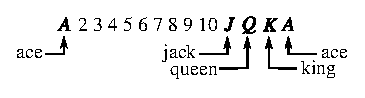
\includegraphics{figure/fig1.eps}}
\end{frame}

\begin{frame}
There are $\binom{52}{5}$ (five-card) poker hands.
\begin{enumerate}
\item $A=\dfrac{A \text{~``Straight''}}{\substack{\text{all five cards are}\\ \text{consecutive = a ``straight''}}}$
\end{enumerate}

e.g., $56789$.

or $A2345$ aces are low

or $10JQKA$ aces are high.

Find $P(A)$, this is Problem 43 from the text.

There is one observation you need -

{\it a straight is almost determined by its bottom (i.e., lowest) card.}
\end{frame}

\begin{frame}
You need one more sub observation: the cards.

cards, \underline{$J$, $Q$, $K$} cannot be bottom cards for a straight (because there aren't enough cards above them).

The last straight is 

$10 \ \ J \ \ K \ \ Q \ \ A \longleftarrow$ aces are high.

Also $A$ can be a bottom card because aces are low
$$
A~~2~~3~~4~~5
$$
So there are $13-3=10$ bottom cards so there are 10 different kinds of straights - so at first glance one might think 
\end{frame}

\begin{frame}
there are 10 straights. But, let's consider $A2345$. We haven't taken account of the SUITS of the cards. The $A$ could be any one of four suits, for each of these the 2 could be any one of four suits so there are $4^{5}$ straights of the form $AZ345$. Hence

\medskip
\centerline{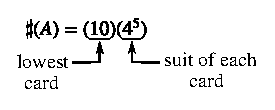
\includegraphics{figure/fig2.eps}}
\smallskip

So
$$
P(A)=\dfrac{(10)(4^{5})}{\binom{52}{5}}
$$
\end{frame}

\begin{frame}
\myheading{2. A ``Flush''}

A ``flush'' is a poker hand in which all cards are of the same suit (spade, heart, diamond or club).

Let $B$ = set of all flushes.

First - how many hands are there that are all hearts?

We use the principle of restricted choice. There are 13 hearts, we have to choose 5. So there are $\binom{13}{5}$ such hands. So we have

\medskip
\centerline{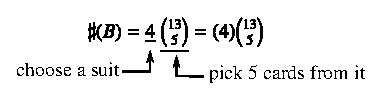
\includegraphics{figure/fig3.eps}}
\end{frame}

\begin{frame}
So
$$
P(B)=\dfrac{(4)\binom{15}{5}}{\binom{52}{5}}
$$

\myheading{3. A ``Straight Flush''}

Lets combine 2 and 3. So 

$C$ = set of all straights so that all the cards have the same suit.

To compute $\sharp(C)$ first pick the lowest card\qquad 10 ways

then

pick the suit that all five cards have\qquad 4 ways

So \ \ $\sharp(C)=(10)(4)=40$
$$
\text{and}\quad P(C)=\dfrac{40}{\binom{52}{5}}=\text{a very small number}
$$
\end{frame}

\begin{frame}
\myheading{4. A Full House}

A full house is a poker hand which consists of 3 of one kind and 2 of a different kind e.g., $JJJ~KK$.

Let $D$ = set of full houses.

Here is how we compute $\sharp(D)$.
\begin{enumerate}
\item Pick an {\it ordered} pair of kinds e.g., $J$ or $K$.

\item Pick 3 of the first and 2 of the second.
\end{enumerate}
\end{frame}

\begin{frame}
So in the above case we get $JJJ~KK$.

\myheading{Key test to perform}

Were we right when we said ORDERED pair above?

So let's test, reverse the order $K$, $J$ and check if we get a different hand.

If we do we were right to say ORDERED pairs.

If we don't we were wrong and we have to replace ORDERED pairs in $1$. by UNORDERED pairs.
\end{frame}

\begin{frame}
Okay if we take the pair $K$, $J$ and do $2$.

We get the hand $KKK~JJ$ are $KKK~JJ$ and $JJJ~KK$ different? {\it yes}, the first beats the second so we were right to pick ordered pairs.

Now lets finish the job
\begin{enumerate}
\item There are 13 kinds, so ordered pair of kinds is a 2 permutation of the 13 element set of kinds.

So.
\begin{align*}
\sharp(1.) &= P_{2,13}=\dfrac{(13)!}{(11)!}\\[4pt]
           &= (13)(12)
\end{align*}
\end{enumerate}
\end{frame}

\begin{frame}
\begin{enumerate}
\setcounter{enumi}{1}
\item Now there are $\binom{4}{3}$ to pick the first kind (say the first kind is a jack so we have to pick 3 of the 4 jacks) and $\binom{4}{2}$ ways to pick the second kind so
$$
\sharp(D)=\underbrace{(13)(12)}_{2\text{~kinds}}\binom{4}{3}\binom{4}{2}
$$
so
$$
P(D)=\dfrac{(13)(12)\binom{4}{3}\binom{4}{2}}{\binom{52}{5}}
$$
\end{enumerate}
\end{frame}

\begin{frame}
\myheading{4. Two Pair}

In poker ``two pair'' is a hand which consists of 2 of one kind, 2 of a second ({\it different}) kind and one more of a third kind ({\it different} from the other two)

e.g., $JJ~KK10$

Let $E$ be the set of two - pair hands. Here is how we compute $\sharp(E)$.
\begin{enumerate}
\item Pick an \ \ $\left\{\begin{array}{l} ordered\\ unordered\end{array}\right.$ \ \ pair of kinds.

e.g., $J$, $K$.

\item Pick a third kind.

\item Pick two each of the first two kinds and one of the 
\end{enumerate}
\end{frame}

\begin{frame}
third kind.

\myheading{64,000 Question}

In 1. do we pick an {\it ordered} pair or an {\it unordered} pain?

{\it Answer} Do the test?

The pair $J$, $K\longrightarrow JJKK$

The pair $K$, $J\longrightarrow KkJJ$

In poker $JJKK$ and $KKJJ$ are the {\it SAME} so $J$, $K$ and $K$, $J$ give the {\it SAME} hand so order does not matter.

So we pick an {\it unordered} pain.
\end{frame}

\begin{frame}
Now we compute $\sharp(E)$.
\begin{enumerate}
\item There are 13 kinds.

We want the number of {\it unordered} pairs. It is $\binom{13}{2}=\dfrac{(13)(12)}{2}$

$=\dfrac{1}{2}$ \ \ the number we get for 1. in the full house case.

\item We have chosen two kinds. There are $13-2=11$ left. We have to pick one so
$\binom{11}{1}=11$.
\end{enumerate}
\end{frame}

\begin{frame}
\begin{enumerate}
\setcounter{enumi}{2}
\item $\binom{4}{2}=6$ for the first kind.

$\binom{4}{2}=6$ for the second kind.
\end{enumerate}
(there is no first or second but it does matter the numbers are the same) $\binom{4}{1}=4$ for the third kind.
$$
\sharp(t)=\left(\dfrac{(13)(12)}{2}\right)(11)\binom{4}{2}\binom{4}{2}(4)
$$
so
$$
P(E)=\dfrac{\left(\frac{(13)(12)}{2}\right)(11)(6)(6)(4)}{\binom{52}{5}}
$$
\end{frame}

\end{document}


